\section{The subgraphs $F(x)$ and the graphs $F_m$}\label{sec:F}

For $x\ge2$ let $D(x)=\{N\ge2:N\mid x\}$, so $|D(x)|=\tau(x)-1=:b$, and for $N\in D(x)$ put $y_N=x\,r_N=x(N+1)^2/N$. Define $F(x)$ to be the graph with vertices $x,\,4x$, and $y_N,\,4y_N$ ($N\in D(x)$), and edges
\[
x\!-\!4x,\qquad x\!-\!y_N,\qquad y_N\!-\!4y_N,\qquad 4y_N\!-\!4x\qquad(N\in D(x)).
\]
Write $F_m=F(2^m)$. Here $D(2^m)=\{2,4,\dots,2^m\}$, so with $N=2^j$,
\[
y_j=2^{m-j}(2^j+1)^2\quad(1\le j\le m).
\]

\begin{figure}[t]
\centering
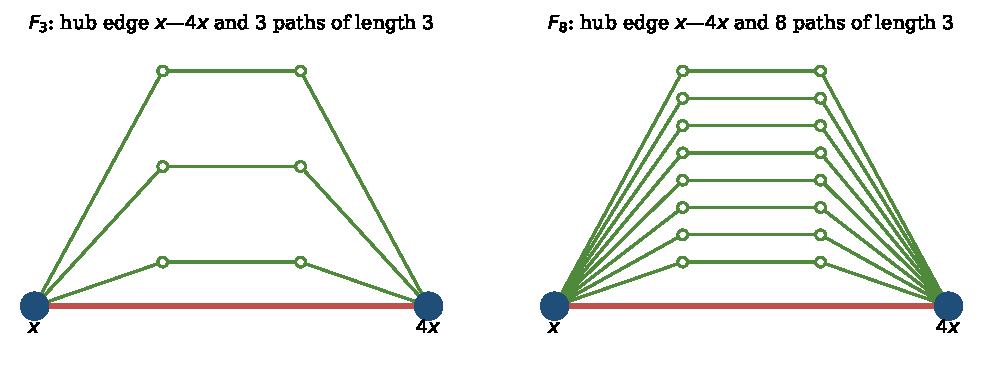
\includegraphics[width=0.92\textwidth]{../figures/fig2_Fm_theta.pdf}
\caption{The graphs $F_3$ and $F_8$: a hub edge $x\!-\!4x$ (red) and $m$ internally disjoint paths of length $3$ (green) between its endpoints. Equivalently, $m$ four-cycles (scaling squares, Theorem~\ref{thm:cycles}(iv)) sharing the edge $x\!-\!4x$: the book graph with $m$ pages.}\label{fig:Fm}
\end{figure}

\begin{figure}[t]
\centering
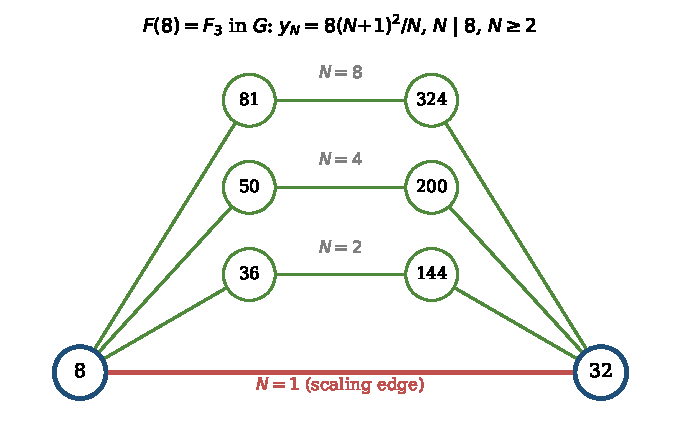
\includegraphics[width=0.66\textwidth]{../figures/fig3_F8_labelled.pdf}
\caption{$F(8)=F_3$ with its arithmetic labels: $y_N=8(N+1)^2/N$ for $N=2,4,8$ gives $36,\,50,\,81$ and $4y_N=144,\,200,\,324$.}\label{fig:F8}
\end{figure}

\begin{proposition}[Structure of $F(x)$]\label{prop:Fx}
For $x\ge2$ with $b=\tau(x)-1$, $F(x)$ is a subgraph of $G$ and is isomorphic to the theta graph $\Theta(1,3,\dots,3)$ with $b$ paths of length $3$. It has $2b+2$ vertices, $3b+1$ edges, and the hubs $x$, $4x$ have degree $b+1=\tau(x)$.
\end{proposition}
\begin{proof}
\emph{Edges lie in $G$.} $\{x,4x\}$: $k=x,N=1$. $\{x,y_N\}$: $k=x/N$. $\{y_N,4y_N\}$: $k=y_N,N=1$. $\{4x,4y_N\}$: $k=4x/N$ (here $N\mid x$ is used).

\emph{Vertices are distinct.} $x<4x<y_N$ because $r_N>4$ for $N\ge2$; $y_N<4y_N$; the $y_N$ are distinct since $N\mapsto r_N$ is injective, hence so are the $4y_N$. It remains to exclude $y_N=4y_{N'}$ for $N\ne N'$, i.e.\ $r_N=4r_{N'}$. Let $g=\gcd(4,N')\in\{1,2,4\}$; the reduced form of $4r_{N'}$ has denominator $N'/g$ and numerator $4(N'+1)^2/g$, so equality with $r_N$ forces $N'=gN$ and $g(N+1)^2=4(gN+1)^2$. For $g=1$: $(N+1)^2=4(N+1)^2$; for $g=2$: $(N+1)^2=2(2N+1)^2$, impossible as $2N+1>N+1$; for $g=4$: $N+1=4N+1$, so $N=0$. All impossible.

\emph{Theta structure.} The paths $x\!-\!y_N\!-\!4y_N\!-\!4x$ have disjoint interiors, and together with the direct edge they join $x$ to $4x$. Counting gives the stated numbers. \qedhere
\end{proof}

\begin{lemma}[The cubic]\label{lem:cubic}
For $m\ge1$ the equation $\lambda^3-\lambda^2+\lambda=m$ has a unique real root $\lambda_m$; it is increasing in $m$, $\lambda_1=1$, and for $m\ge2$
\[
m^{1/3}<\lambda_m<m^{1/3}+\tfrac13,\qquad
\lambda_m=m^{1/3}+\tfrac13-\tfrac29m^{-1/3}-\tfrac7{81}m^{-2/3}+O(m^{-1}),
\]
\[
\tfrac13\log m<\log\lambda_m<\tfrac13\log m+\frac1{3m^{1/3}} .
\]
\end{lemma}
\begin{proof}
Put $g(\lambda)=\lambda^3-\lambda^2+\lambda-m$; $g'(\lambda)=3\lambda^2-2\lambda+1>0$, so $g$ is strictly increasing, which gives uniqueness and monotonicity in $m$; $g(1)=1-m$ vanishes at $m=1$. Let $t=m^{1/3}>1$ ($m\ge2$). Then $g(t)=-t^2+t<0$, so $\lambda_m>t$, and $g(t+\tfrac13)=\tfrac23t+\tfrac7{27}>0$, so $\lambda_m<t+\tfrac13$. Taking logarithms, $\log\lambda_m<\log t+\log(1+\tfrac1{3t})<\tfrac13\log m+\tfrac1{3t}$. For the expansion substitute $\lambda=t+a+bt^{-1}+ct^{-2}+O(t^{-3})$ into $\lambda^3-\lambda^2+\lambda=t^3$: the coefficients of $t^2,t^1,t^0$ give $3a-1=0$, $3a^2+3b-2a+1=0$, $a^3+6ab+3c-a^2-2b+a=0$, i.e.\ $a=\tfrac13$, $b=-\tfrac29$, $c=-\tfrac7{81}$. \qedhere
\end{proof}

\begin{theorem}[Exact nonbacktracking entropy of $F(x)$]\label{thm:entropy}
For every $x\ge2$, $\hNB(F(x))=\log\lambda_{\tau(x)-1}$. In particular
\[
\hNB(F_m)=\log\lambda_m,\qquad \tfrac13\log m<\hNB(F_m)<\tfrac13\log m+\tfrac{1}{3m^{1/3}}\ (m\ge2),
\]
and $\hNB(F(x))>\tfrac13\log(\tau(x)-1)>\tfrac14\log(\tau(x)-1)$ for $\tau(x)\ge3$. Moreover $\hNB(F(x))\le\log(\tau(x)-1)$.
\end{theorem}
\noindent\emph{Source.} The exact value and the cubic equation are established in this paper. The inherited release~\cite{UENT} gives the lower bound $\tfrac14\log(\tau(x)-1)$ and numerical spectral radii for $F(2^m)$, $2\le m\le9$ (Section~\ref{sec:recon}).
\begin{proof}
Let $b=\tau(x)-1$. If $b=1$, $F(x)$ is a $4$-cycle, $B$ is a permutation matrix and $\hNB=0=\log\lambda_1$. For $b\ge2$, apply Theorem~\ref{thm:theta} with lengths $(1,3,\dots,3)$ ($s=b+1\ge3$): $\lambda=\rho(B)$ is the root $>1$ of $\frac1{\lambda+1}+\frac b{\lambda^3+1}=1$. Since $\lambda^3+1=(\lambda+1)(\lambda^2-\lambda+1)$, this reads $b=\lambda(\lambda^2-\lambda+1)=\lambda^3-\lambda^2+\lambda$, i.e.\ $\lambda=\lambda_b$. The bounds follow from Lemma~\ref{lem:cubic}, $\log\lambda_b>\tfrac13\log b>\tfrac14\log b$ for $b>1$, and the degree bound of Lemma~\ref{lem:mono} with $\Delta=b+1$. \qedhere
\end{proof}

\begin{theorem}[Spectrum of $B_{F_m}$]\label{thm:spectrum}
For $m\ge1$,
\[
\det(\lambda I-B_{F_m})=(\lambda^6-1)^{m-1}(\lambda^2-1)(\lambda^3-\lambda^2+\lambda-m)(\lambda^3+\lambda^2+\lambda+m),
\]
and the Ihara--Bass type determinant is
\[
\det(I-uB_{F_m})=(1-u^6)^{m-1}(1-u^2)(1-u+u^2-mu^3)(1+u+u^2+mu^3).
\]
The spectrum is symmetric about $0$; the spectral radius is $\lambda_m$ and the eigenvalue $-\lambda_m$ is simple.
\end{theorem}
\begin{proof}
Apply Theorem~\ref{thm:spectrum-gen} with $\ell=(1,3^m)$. Then
\[
P_+=(\lambda+1)(\lambda^3+1)^m-(\lambda^3+1)^m-m(\lambda+1)(\lambda^3+1)^{m-1}=(\lambda^3+1)^{m-1}(\lambda+1)(\lambda^3-\lambda^2+\lambda-m),
\]
using $\lambda(\lambda^3+1)-m(\lambda+1)=(\lambda+1)(\lambda^3-\lambda^2+\lambda-m)$, and
\[
P_-=(\lambda-1)(\lambda^3-1)^m+(\lambda^3-1)^m+m(\lambda-1)(\lambda^3-1)^{m-1}=(\lambda^3-1)^{m-1}(\lambda-1)(\lambda^3+\lambda^2+\lambda+m),
\]
using $\lambda(\lambda^3-1)+m(\lambda-1)=(\lambda-1)(\lambda^3+\lambda^2+\lambda+m)$. The product is the stated polynomial. The determinant $\det(I-uB)$ is $u^{2|E|}\det(\lambda I-B)|_{\lambda=1/u}$ with $2|E|=6m+2$. The polynomial $\lambda^3+\lambda^2+\lambda+m=-g(-\lambda)$ has the roots $-\lambda_m$ and the negatives of the other roots of $g$, whose modulus $\sqrt{m/\lambda_m}<\lambda_m$ (product of roots $=m<\lambda_m^3$). \qedhere
\end{proof}

\begin{theorem}[The induced subgraph]\label{thm:induced}
For every $m\ge1$ the subgraph of $G$ induced on $V(F_m)$ equals $F_m$. Consequently $Y_{\mathrm{NB}}(F(2^m))$, the metric shift on the window $G[V(F_m)]$, has entropy $\log\lambda_m$.
\end{theorem}
\begin{proof}
Write $o_j=2^j+1$ (odd), so $y_j=2^{m-j}o_j^2$ and $4y_j=2^{m-j+2}o_j^2$. In $F_m$ the pairs at distance $2$ are $(x,4y_j)$, $(4x,y_j)$, $(y_j,y_k)$, $(4y_j,4y_k)$; any such pair adjacent in $G$ would create a triangle, impossible by Theorem~\ref{thm:cycles}(i). The only other non-adjacent (in $F_m$) pairs are $\{y_j,4y_k\}$ with $j\ne k$ (distance $3$). We show these are non-adjacent in $G$.

Let $P=y_j$, $Q=4y_k$ and let $R>1$ be the ratio of the larger to the smaller. By Lemma~\ref{lem:edges}, $P,Q$ are adjacent iff $R=(q+1)^2/q$ in lowest terms. Say the larger is $2^a o_J^2$ and the smaller $2^bo_K^2$ ($J\ne K$), $e=a-b$, $\gamma=\gcd(o_J,o_K)$, $p=o_J/\gamma$, $r=o_K/\gamma$ (coprime, odd). Then $R=2^ep^2/r^2$.
\begin{itemize}[itemsep=1pt]
\item If $e\ge0$, the reduced numerator is $2^ep^2$ and the denominator $r^2$; adjacency needs $2^ep^2=(r^2+1)^2$. As $r$ is odd, $r^2+1\equiv2\pmod 4$, so $e=2$.
\item If $e=-f<0$, the reduced fraction is $p^2/(2^fr^2)$; adjacency needs $p=2^fr^2+1$.
\end{itemize}
\emph{Case A: $4y_k$ is larger} ($J=k$, $K=j$, $e=j-k+2$). If $e=2$ then $j=k$, excluded. If $e=-f<0$, then $f=k-j-2\ge1$ and $o_k=\gamma+2^fo_j^2/\gamma$. With $o_k=2^{f+j+2}+1$ and $o_j=\gamma r$ this becomes
\[
\gamma-1=2^f\bigl(2^{j+2}-(2^j+1)r\bigr).
\]
If $\gamma=1$ the right side must vanish, but $(2^j+1)r$ is odd and $2^{j+2}$ is even. So $\gamma>1$ and $(2^j+1)r<2^{j+2}$, whence $r\in\{1,3\}$ ($r=3$ needs $j\ge2$) and $D:=2^{j+2}-(2^j+1)r$ is odd. For $r=1$: $\gamma=o_j$, $2^j=2^f(3\cdot2^j-1)$, impossible as $3\cdot2^j-1$ is an odd divisor of $2^j$ exceeding $1$. For $r=3$: $\gamma=(2^j+1)/3$ and $(2^j-2)/3=2^f(2^j-3)$, so $2^j-2\ge6(2^j-3)$, i.e.\ $2^j\le3$, contradicting $j\ge2$.

\emph{Case B: $y_j$ is larger} ($J=j$, $K=k$, $e=k-j-2$). If $e=2$ then $k=j+4$ and $R=4o_j^2/o_k^2<1$ because $o_k>2o_j$; contradiction. If $e=-f<0$ then $f=j-k+2\ge1$ and $o_j=\gamma+2^fo_k^2/\gamma\ge2^fo_k=2^{j+2}+2^{j-k+2}>2^j+1=o_j$ (since $\gamma\mid o_k$), a contradiction.

Hence $G[V(F_m)]=F_m$. The last assertion follows from the remark on $Y_{\mathrm{NB}}$ in Section~\ref{sec:nb} and Theorem~\ref{thm:entropy}. \qedhere
\end{proof}


\begin{example}[The three smallest cases]\label{ex:small}
\emph{$F_2=F(4)$.} $D(4)=\{2,4\}$, $y_2=4\cdot\tfrac92=18$, $y_4=4\cdot\tfrac{25}4=25$; the vertices are $4,16,18,72,25,100$ and the edges $4\!-\!16$, $4\!-\!18$, $18\!-\!72$, $72\!-\!16$, $4\!-\!25$, $25\!-\!100$, $100\!-\!16$ (labels: $N=1$ for $\{4,16\}$, $\{18,72\}$, $\{25,100\}$; $N=2$ for $\{4,18\}$ with $k=2$ and $\{16,72\}$ with $k=8$; $N=4$ for $\{4,25\}$ with $k=1$ and $\{16,100\}$ with $k=4$).

\emph{$F_3=F(8)$} (Figure~\ref{fig:F8}): $x=8$, $4x=32$, $y=36,50,81$ and $4y=144,200,324$. The six pairs $\{y_j,4y_k\}$, $j\ne k$, which Theorem~\ref{thm:induced} must exclude, have ratios $200/36=50/9$, $324/36=9$, $144/50=72/25$, $324/50=162/25$, $144/81=16/9$, $200/81$. Since adjacency requires a ratio $(q+1)^2/q$ in lowest terms, with denominator $q$ and numerator $(q+1)^2$, none of these is an edge: $50/9$ would need $q=9$ and numerator $100$; $9=9/1$ would need $q=1$ and numerator $4$; $72/25$ needs numerator $676$; $162/25$ needs $676$; $16/9$ needs $100$; $200/81$ needs $6724$.

\emph{$F(12)$, a composite $x$.} $\tau(12)=6$, $D(12)=\{2,3,4,6,12\}$, $y_N=12r_N=54,64,75,98,169$. The graph $F(12)\cong\Theta(1,3^5)$ has the $12$ vertices $12,48,54,216,64,256,75,300,98,392,169,676$ and entropy $\log\lambda_5=0.6319\ldots$ (Theorem~\ref{thm:entropy}).
\end{example}

\section{Symbolic transition matrices, periodic paths and the maximal-entropy measure}\label{sec:symbolic}

\paragraph{Transition matrices.}
By the proof of Theorem~\ref{thm:spectrum-gen}, $B_{F_m}$ is similar to $B_+\oplus B_-$, where $B_\varepsilon$ acts on the $3m+1$ coordinates $(D;P_1^1,P_1^2,P_1^3;\dots;P_m^1,P_m^2,P_m^3)$ (the direct edge $D$ and the three edges of each path $P_i$, counted from the hub where the walk enters) by
\[
D\to P_i^1\ (\varepsilon),\qquad P_i^1\to P_i^2\to P_i^3,\qquad P_i^3\to D,\ P_k^1\ (k\ne i)\ (\varepsilon).
\]
For $m=2$:
\[
B_+=\setlength{\arraycolsep}{2pt}\left(\begin{array}{ccccccc}0 & 1 & 0 & 0 & 1 & 0 & 0\\0 & 0 & 1 & 0 & 0 & 0 & 0\\0 & 0 & 0 & 1 & 0 & 0 & 0\\1 & 0 & 0 & 0 & 1 & 0 & 0\\0 & 0 & 0 & 0 & 0 & 1 & 0\\0 & 0 & 0 & 0 & 0 & 0 & 1\\1 & 1 & 0 & 0 & 0 & 0 & 0\end{array}\right)
\]
\[
B_-=\setlength{\arraycolsep}{2pt}\left(\begin{array}{ccccccc}0 & -1 & 0 & 0 & -1 & 0 & 0\\0 & 0 & 1 & 0 & 0 & 0 & 0\\0 & 0 & 0 & 1 & 0 & 0 & 0\\-1 & 0 & 0 & 0 & -1 & 0 & 0\\0 & 0 & 0 & 0 & 0 & 1 & 0\\0 & 0 & 0 & 0 & 0 & 0 & 1\\-1 & -1 & 0 & 0 & 0 & 0 & 0\end{array}\right)
\]
and $\det(\lambda I-B_\pm)=P_\pm$ (checked symbolically).

\paragraph{The label shift.}
A walk in $F_m$ is forced through each path once it has entered it (the interior vertices have degree $2$), so a bi-infinite NB walk is a sequence of full traversals $w_i\in\{D,1,\dots,m\}$ with $w_i\ne w_{i+1}$ (leaving a hub, the walk may take any path other than the one just used). The label transfer matrix with weights $u^{\mathrm{length}}$, $\mathrm{length}(D)=1$, $\mathrm{length}(i)=3$, is $T(u)_{ij}=[i\ne j]u^{\ell_j}$; for $m=3$,
\[
T(u)=\left[\begin{matrix}0 & u^{3} & u^{3} & u^{3}\\u & 0 & u^{3} & u^{3}\\u & u^{3} & 0 & u^{3}\\u & u^{3} & u^{3} & 0\end{matrix}\right].
\]
\begin{remark}\label{rem:T}
If $c_i=X/(\mu+x_i)$ with $x_i=u^{\ell_i}$, $X=\sum x_ic_i$, then $T(u)c=\mu c$; summing shows that the Perron eigenvalue $\mu=1$ occurs iff $\sum_ix_i/(1+x_i)=1$, which for $u=1/\lambda$ is the equation $\sum_i(\lambda^{\ell_i}+1)^{-1}=1$ of Theorem~\ref{thm:theta}. So $\lambda_m^{-1}$ is the value of $u$ at which the weighted label shift has spectral radius $1$: the NB shift of $F_m$ is the suspension of the no-immediate-repetition shift on $m+1$ symbols with roof function $\ell_D=1$, $\ell_i=3$.
\end{remark}

\begin{theorem}[Periodic symbolic paths]\label{thm:periodic}
Let $m\ge2$.
\begin{enumerate}[label=(\roman*),itemsep=1pt]
\item The simple cycles of $F_m$ are exactly $m$ cycles of length $4$ (the direct edge plus one path) and $\binom m2$ cycles of length $6$ (two paths).
\item The number of periodic points of period $n$ of the NB shift (closed NB walks of length $n$ with marked start and orientation) is
\[
\tr B^n=6(m-1)\,[6\mid n]+\bigl(1+(-1)^n\bigr)(1+s_n),
\]
where $s_n=\sum_\lambda\lambda^n$ over the roots of $\lambda^3-\lambda^2+\lambda-m$, i.e.\ $s_0=3$, $s_1=1$, $s_2=-1$, $s_n=s_{n-1}-s_{n-2}+ms_{n-3}$. In particular $\tr B^4=8m$, $\tr B^6=6m(m-1)$, $\tr B^n=0$ for odd $n$, and $\tr B^n=2\lambda_m^n+O\bigl((m/\lambda_m)^{n/2}\bigr)$ for even $n$.
\item $\limsup_n\frac1n\log\tr B^n=\log\lambda_m=\hNB(F_m)$.
\end{enumerate}
\end{theorem}
\begin{proof}
(i) Every vertex other than the hubs has degree $2$, so a simple cycle containing one interior vertex contains the whole path and both hubs, hence consists of exactly two of the $m+1$ paths. Pairs $\{D,P_i\}$ give length $1+3=4$; pairs $\{P_i,P_j\}$ give $3+3=6$.

(ii) $\tr B^n=\sum\mu^n$ over the eigenvalues. Theorem~\ref{thm:spectrum} gives: the $6$th roots of unity, each with multiplicity $m-1$, contribute $6(m-1)[6\mid n]$; $\pm1$ contribute $1+(-1)^n$; the roots of $g$ contribute $s_n$ and those of $\lambda^3+\lambda^2+\lambda+m$, the negatives of these, contribute $(-1)^ns_n$. Newton's identities give the recursion. $\tr B^4=8m$ counts $2\cdot4$ rotations/orientations for each of the $m$ four-cycles, and $\tr B^6=6m(m-1)$ is $12\binom m2$. The error term follows from $|z|^2=m/\lambda_m<\lambda_m^2$ for the two non-real roots $z$ of $g$.

(iii) follows from (ii) with $n$ even. \qedhere
\end{proof}

\begin{table}[h]
\centering\small
\begin{tabular}{rrrrrrrrr}\toprule $m$ & $n{=}4$ & $6$ & $8$ & $10$ & $12$ & $14$ & $16$ & $18$\\\midrule
2 & 16 & 12 & 32 & 40 & 76 & 168 & 192 & 588\\
3 & 24 & 36 & 72 & 240 & 324 & 1512 & 2184 & 8172\\
4 & 32 & 72 & 128 & 720 & 1016 & 6048 & 12416 & 45864\\
5 & 40 & 120 & 200 & 1600 & 2560 & 16800 & 45960 & 168600\\
6 & 48 & 180 & 288 & 3000 & 5508 & 37800 & 130368 & 482580\\
\bottomrule\end{tabular}

\caption{Numbers $\tr B^n$ of periodic NB points of period $n$ for $F_m$ (odd $n$ give $0$).}\label{tab:trace}
\end{table}

\begin{table}[h]
\centering\small
\begin{tabular}{rrrrrrrrr}\toprule $m$ & $\pi_4$ & $\pi_6$ & $\pi_8$ & $\pi_{10}$ & $\pi_{12}$ & $\pi_{14}$ & $\pi_{16}$ & $\pi_{18}$\\\midrule
2 & 4 & 2 & 2 & 4 & 4 & 12 & 10 & 32\\
3 & 6 & 6 & 6 & 24 & 22 & 108 & 132 & 452\\
4 & 8 & 12 & 12 & 72 & 76 & 432 & 768 & 2544\\
5 & 10 & 20 & 20 & 160 & 200 & 1200 & 2860 & 9360\\
6 & 12 & 30 & 30 & 300 & 440 & 2700 & 8130 & 26800\\
\bottomrule\end{tabular}

\caption{Numbers $\pi_n=\frac1n\sum_{d\mid n}\mu(n/d)\tr B^d$ of primitive periodic NB orbits of length $n$ in $F_m$ (all entries are non-negative integers).}\label{tab:prime}
\end{table}

\begin{figure}[t]
\centering
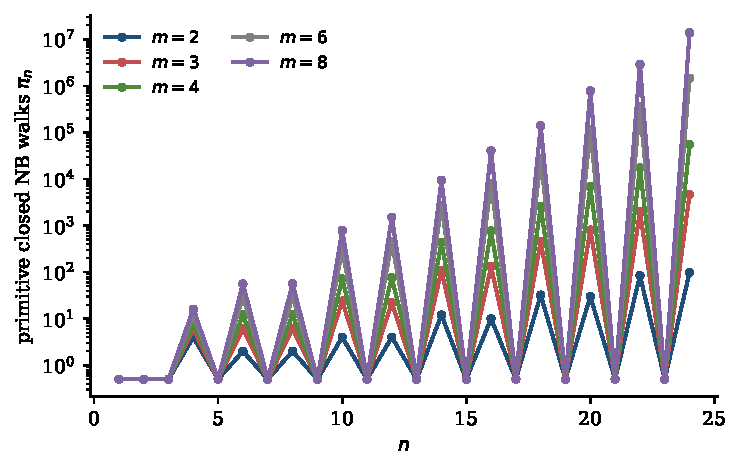
\includegraphics[width=0.78\textwidth]{../figures/fig7_periodic_counts.pdf}
\caption{Numbers of primitive periodic orbits of the NB shift of $F_m$ for $m=2,3,4,6,8$ (logarithmic scale; odd periods have none and are drawn at $1/2$).}\label{fig:periodic}
\end{figure}

\paragraph{Maximal-entropy measure.}
For $m\ge2$, $B_{F_m}$ is irreducible: from any directed edge, at the end of its path there are $m+1\ge3$ paths available at the hub, so any directed edge can be reached after at most two further full traversals. Let $\varphi$ be the positive eigenvector of Theorem~\ref{thm:theta}; with the normalisation $b=\varphi(P^1_i)=1$ one has $a=\varphi(D)=m/\lambda$ (because $(\lambda^3+1)/(\lambda+1)=\lambda^2-\lambda+1=m/\lambda$) and $\varphi(P^t_i)=\lambda^{t-1}$.

\begin{proposition}[Maximal-entropy chain]\label{prop:chain}
The Markov measure with transition probabilities $\mathsf P(e,e')=\varphi(e')/(\lambda\varphi(e))$ on $\vec E(F_m)$ is the unique measure of maximal entropy of $X_{\mathrm{NB}}(F_m)$ and has entropy $\log\lambda_m$. Its transitions are: probability $1$ along the interior of a path; from the direct edge to each of the $m$ paths, $1/m$; from the end of a path to the direct edge, $m/\lambda_m^4$, and to each of the other $m-1$ paths, $\lambda_m^{-3}$.
\end{proposition}
\begin{proof}
For $B\varphi=\lambda\varphi$, $\varphi>0$, the matrix $\mathsf P$ is stochastic; $-\sum\pi(e)\mathsf P(e,e')\log\mathsf P(e,e')=\log\lambda+\sum\pi(e)\mathsf P(e,e')(\log\varphi(e)-\log\varphi(e'))=\log\lambda$ for the stationary $\pi$. Since $\hNB=\log\lambda$ this is the maximal entropy, and uniqueness is the Parry theorem for irreducible matrices (a periodic irreducible matrix still has a unique measure of maximal entropy). The values: from $D$, $\varphi(P_i^1)/(\lambda a)=b/(m b)=1/m$; from the end $P_i^3$, $\varphi=\lambda^2$, so $\mathsf P\to D$ is $a/\lambda^3=m/\lambda^4$ and $\mathsf P\to P_k^1$ is $1/\lambda^3$. These sum to $1$ because $m+(m-1)\lambda=\lambda^4$, which follows from $\lambda^3=m+\lambda^2-\lambda$. \qedhere
\end{proof}

\begin{figure}[t]
\centering
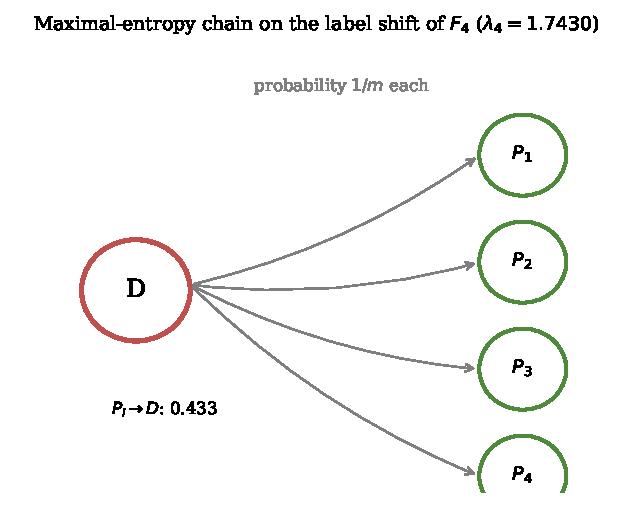
\includegraphics[width=0.58\textwidth]{../figures/fig8_chain.pdf}
\caption{Branching of the maximal-entropy chain on $F_4$ ($\lambda_4=1.7430$): at the hub after the direct edge each path has probability $1/m$; after a path the walk returns along the direct edge with probability $m/\lambda_m^4$.}\label{fig:chain}
\end{figure}


\paragraph{Why the reversal symmetry matters.}
The reversal $e\mapsto\bar e$ satisfies $B(e,e')=B(\bar e',\bar e)$, so $B^\top=RBR$ where $R$ is the permutation matrix of reversal. Hence if $B\varphi=\lambda\varphi$ then $\psi(e):=\varphi(\bar e)$ satisfies $\psi^\top B=\lambda\psi^\top$: the left Perron vector is the reversed right Perron vector.

\begin{proposition}[Stationary distribution]\label{prop:stationary}
For $m\ge2$ the stationary distribution of the maximal-entropy chain is $\pi(e)=\varphi(e)\varphi(\bar e)/Z$. It is \emph{constant along each path}: all six directed edges of a $3$-path carry mass $\lambda_m^2/Z$ and the two directed copies of the direct edge carry $m^2/(\lambda_m^2Z)$ each, where $Z=2m^2/\lambda_m^2+6m\lambda_m^2$ (normalisation $\varphi(P_i^1)=1$). In particular the proportion of time spent on the direct edge is
\[
\frac{m}{m+3\lambda_m^4},
\]
which tends to $0$ like $3^{-1}m^{-1/3}$; the remaining mass is shared equally among the $m$ paths.
\end{proposition}
\begin{proof}
Since $\psi$ is the left Perron vector, $\pi=\varphi\psi/\psi^\top\varphi$ is the stationary distribution of $\mathsf P(e,e')=\varphi(e')/(\lambda\varphi(e))$ (check: $\sum_e\pi(e)\mathsf P(e,e')=\sum_e\psi(e)B(e,e')\varphi(e')/(\lambda Z)=\psi(e')\varphi(e')/Z$). For the $t$-th edge $e$ of a $3$-path traversed in one direction, $\bar e$ is its $(4-t)$-th edge in the other direction, so $\varphi(e)\varphi(\bar e)=\lambda^{t-1}\lambda^{3-t}=\lambda^2$ independently of $t$. For the direct edge, $\varphi(e)\varphi(\bar e)=(m/\lambda)^2$. Summing over the $6m$ path edges and the $2$ direct edges gives $Z$, and the direct-edge mass $2(m/\lambda)^2/Z=m^2/(m^2+3m\lambda^4)=m/(m+3\lambda^4)$. \qedhere
\end{proof}

\begin{theorem}[Subdominant spectrum and spectral gap]\label{thm:gap}
For $m\ge2$ the eigenvalues of $B_{F_m}$ of maximal modulus are $\pm\lambda_m$ (simple); all other eigenvalues have modulus at most
\[
\sqrt{m/\lambda_m}\;=\;\lambda_m\sqrt{1-\lambda_m^{-1}+\lambda_m^{-2}},
\]
attained by the two non-real roots of $\lambda^3-\lambda^2+\lambda-m$ and of $\lambda^3+\lambda^2+\lambda+m$. Moreover $1<\sqrt{m/\lambda_m}<\lambda_m$.
\end{theorem}
\begin{proof}
By Theorem~\ref{thm:spectrum} the eigenvalues are: the sixth roots of unity and $\pm1$ (modulus $1$), the roots of $g$, and their negatives. The real root of $g$ is $\lambda_m$; the other two roots $z,\bar z$ satisfy $|z|^2=m/\lambda_m$ because the product of the roots is $m$. Then $|z|^2/\lambda_m^2=m/\lambda_m^3=(\lambda_m^3-\lambda_m^2+\lambda_m)/\lambda_m^3=1-\lambda_m^{-1}+\lambda_m^{-2}<1$ because $\lambda_m>1$, and $|z|^2=m/\lambda_m>1$ because $m=\lambda_m^3-\lambda_m^2+\lambda_m>\lambda_m$. \qedhere
\end{proof}
Thus the ratio of subdominant to dominant modulus is $\sqrt{1-\lambda_m^{-1}+\lambda_m^{-2}}\approx1-\tfrac1{2\lambda_m}$ and tends to $1$ as $m\to\infty$ (Figure~\ref{fig:gapmass}): the gap closes at the rate $\tfrac12m^{-1/3}$, while the entropy grows. A further consequence is that the $\sigma$-even and $\sigma$-odd sectors $B_\pm$ of Section~\ref{sec:symbolic} carry the dominant eigenvalues $\lambda_m$ ($B_+$) and $-\lambda_m$ ($B_-$) respectively.

\begin{figure}[t]
\centering
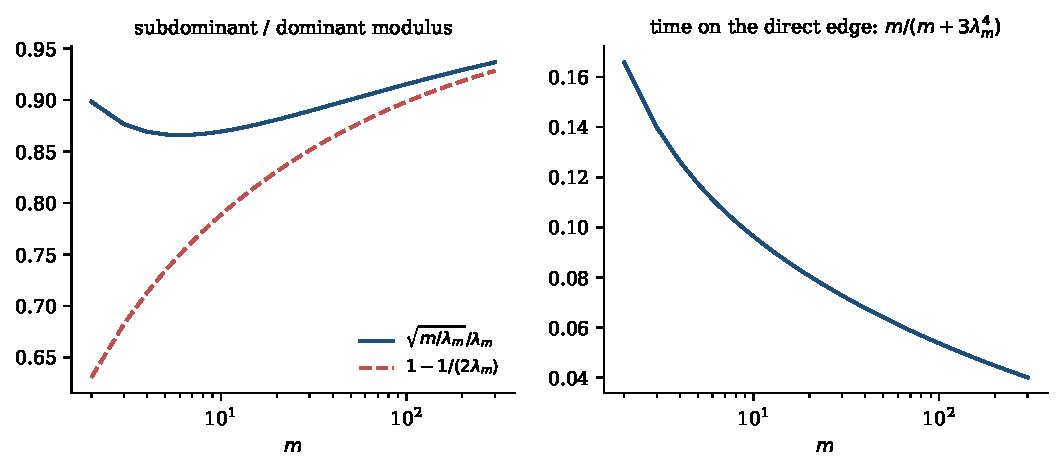
\includegraphics[width=0.95\textwidth]{../figures/fig12_gap_mass.pdf}
\caption{Left: the ratio of subdominant to dominant modulus $\sqrt{m/\lambda_m}/\lambda_m=\sqrt{1-\lambda_m^{-1}+\lambda_m^{-2}}$ (blue) against $1-1/(2\lambda_m)$ (red dashed). Right: the proportion of time $m/(m+3\lambda_m^4)$ spent on the direct edge.}\label{fig:gapmass}
\end{figure}

\paragraph{Counting nonbacktracking histories.}
Let $a_n=\one^\top B^{n-1}\one$ be the number of NB walks with $n$ edges. By Lemma~\ref{lem:CW}, $a_n\asymp\lambda_m^n$, and the ratios $\sqrt{a_{n+2}/a_n}$ converge to $\lambda_m$ (the factor $2$ in the step removes the parity oscillation caused by the eigenvalue $-\lambda_m$); see Table~\ref{tab:counts} and Figure~\ref{fig:ratios}.
\begin{table}[h]
\centering\small
\begin{tabular}{rrrrrrrrrrr}\toprule $m$ & $a_1$ & $a_2$ & $a_3$ & $a_4$ & $a_5$ & $a_6$ & $a_7$ & $a_8$ & $a_9$ & $a_{10}$\\\midrule
2 & 14 & 20 & 28 & 36 & 48 & 68 & 92 & 120 & 164 & 228\\
3 & 20 & 36 & 60 & 84 & 132 & 228 & 348 & 516 & 852 & 1380\\
4 & 26 & 56 & 104 & 152 & 272 & 536 & 872 & 1424 & 2696 & 4760\\
\bottomrule\end{tabular}

\caption{Numbers $a_n$ of nonbacktracking walks of length $n$ in $F_m$.}\label{tab:counts}
\end{table}
\begin{figure}[t]
\centering
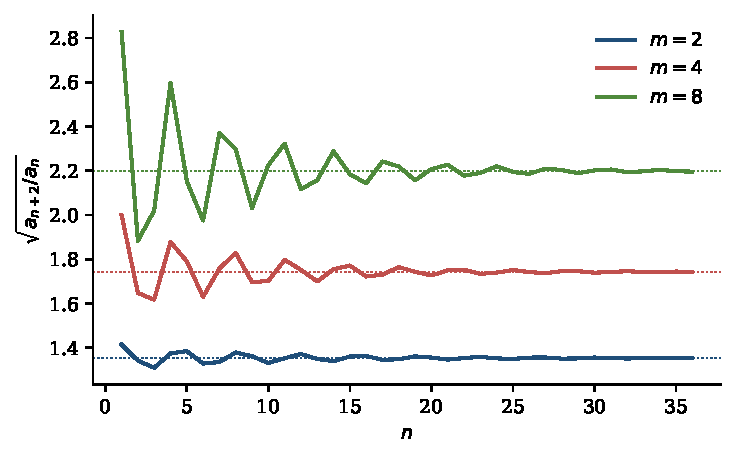
\includegraphics[width=0.62\textwidth]{../figures/fig13_count_ratios.pdf}
\caption{$\sqrt{a_{n+2}/a_n}$ for $m=2,4,8$ against $\lambda_m$ (dotted).}\label{fig:ratios}
\end{figure}

\section{Capacity and asymptotics}\label{sec:capacity}

\begin{theorem}[Unbounded intrinsic history capacity]\label{thm:capacity}
$\Hfin(G)=+\infty$. More precisely:
\begin{enumerate}[label=(\roman*),itemsep=1pt]
\item for every $x\ge2$ the finite subgraph $F(x)\subseteq G$ satisfies $\hNB(F(x))=\log\lambda_{\tau(x)-1}\ge\tfrac13\log(\tau(x)-1)$;
\item $F(x)\subseteq G[1,X]$ whenever $X\ge4(x+1)^2$, hence $\hNB(G[1,X])\ge\tfrac13\log(\tau(x)-1)$ for such $x$; in particular, for $X\ge36$ and $m=\lfloor\log_2(\tfrac12\sqrt X-1)\rfloor$, $\hNB(G[1,X])\ge\tfrac13\log m\to\infty$ as $X\to\infty$;
\item for every $C>0$ and $m>e^{3C}$, $\hNB(F_m)>C$, and the number of NB paths of length $n$ in $F_m$ is at least $\lambda_m^{\,n}\,\one^\top\varphi/\max\varphi$.
\end{enumerate}
\end{theorem}
\noindent\emph{Source.} The inherited argument (Theorem E1 of~\cite{UENT}) concatenates the blocks of $F(x)$ to obtain $\sup_F h\ge\tfrac14\log b(x)=\infty$. The exact capacity statement above, with the bound $\tfrac13\log(\tau(x)-1)$ and the window bounds, is proved in this paper without using that theorem.
\begin{proof}
(i) is Theorem~\ref{thm:entropy}. (ii) $y_N=x(N+1)^2/N$ increases with $N$, so the largest vertex of $F(x)$ is $4y_x=4(x+1)^2$. Monotonicity (Lemma~\ref{lem:mono}) gives the bound on the induced window. For $x=2^m$ one has $\tau(x)-1=m$ and $4(2^m+1)^2\le X$ iff $m\le\log_2(\tfrac12\sqrt X-1)$. (iii) $\log\lambda_m>\tfrac13\log m>C$ for $m>e^{3C}$; the count is Lemma~\ref{lem:CW}. \qedhere
\end{proof}

\begin{figure}[t]
\centering
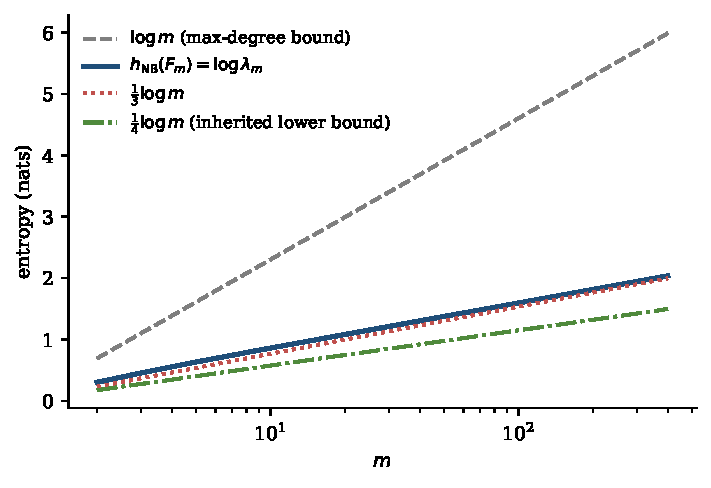
\includegraphics[width=0.78\textwidth]{../figures/fig4_entropy_curves.pdf}
\caption{$\hNB(F_m)=\log\lambda_m$ (blue) between $\tfrac13\log m$ (red dotted) and the degree bound $\log m$ (grey dashed); the inherited bound $\tfrac14\log m$ (green) lies below.}\label{fig:ent}
\end{figure}

\begin{table}[h]
\centering\small
\begin{tabular}{rrrrrr}\toprule $m$ & $\lambda_m$ & $\log\lambda_m$ & $\tfrac13\log m$ & $\tfrac14\log m$ & $\log m$\\\midrule
1 & 1.000000 & 0.000000 & 0.000000 & 0.000000 & 0.000000\\
2 & 1.353210 & 0.302480 & 0.231049 & 0.173287 & 0.693147\\
3 & 1.574743 & 0.454092 & 0.366204 & 0.274653 & 1.098612\\
4 & 1.742959 & 0.555584 & 0.462098 & 0.346574 & 1.386294\\
5 & 1.881239 & 0.631931 & 0.536479 & 0.402359 & 1.609438\\
6 & 2.000000 & 0.693147 & 0.597253 & 0.447940 & 1.791759\\
8 & 2.199280 & 0.788130 & 0.693147 & 0.519860 & 2.079442\\
10 & 2.365019 & 0.860786 & 0.767528 & 0.575646 & 2.302585\\
16 & 2.750859 & 1.011913 & 0.924196 & 0.693147 & 2.772589\\
32 & 3.429364 & 1.232375 & 1.155245 & 0.866434 & 3.465736\\
64 & 4.272298 & 1.452152 & 1.386294 & 1.039721 & 4.158883\\
128 & 5.325490 & 1.672505 & 1.617343 & 1.213008 & 4.852030\\
256 & 6.645784 & 1.893983 & 1.848392 & 1.386294 & 5.545177\\
1024 & 10.389802 & 2.340825 & 2.310491 & 1.732868 & 6.931472\\
\bottomrule\end{tabular}

\caption{The exact entropies $\log\lambda_m$ of $F_m$ against the bounds.}\label{tab:lambda}
\end{table}

\begin{figure}[t]
\centering
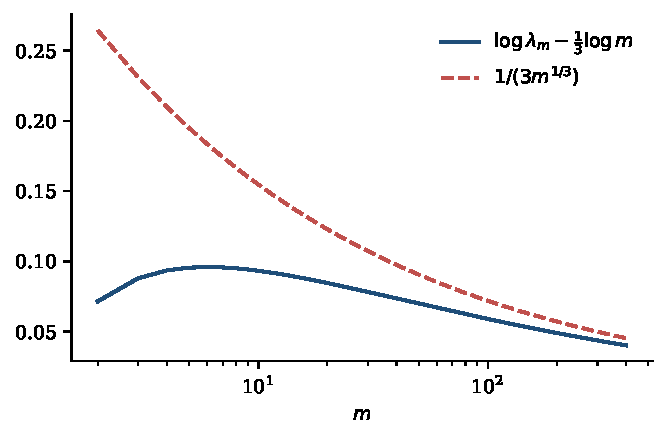
\includegraphics[width=0.48\textwidth]{../figures/fig5_gap.pdf}\hfill
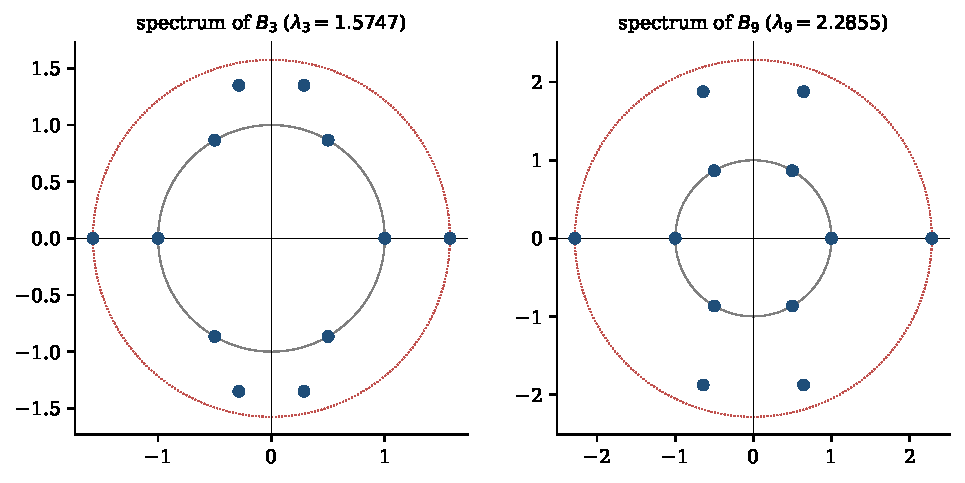
\includegraphics[width=0.48\textwidth]{../figures/fig6_spectrum.pdf}
\caption{Left: $\log\lambda_m-\tfrac13\log m$ against $1/(3m^{1/3})$. Right: spectra of $B_{F_3}$ and $B_{F_9}$ in the complex plane (unit circle in grey; circle of radius $\lambda_m$ dotted).}\label{fig:gapspec}
\end{figure}

\paragraph{Finite windows.}
Theorem~\ref{thm:capacity}(ii) can be sharpened by using the actual divisor function: for each $X$ choose $x$ with $4(x+1)^2\le X$ maximising $\tau(x)$; then $\hNB(G[1,X])\ge\log\lambda_{\tau(x)-1}$. Table~\ref{tab:windowbound} compares this proved bound with the computed value $\log\rho(B)$ of the explicit edge matrix of the window (sparse power iteration); the bound holds in every row, and the computed entropies increase with $X$ (Figure~\ref{fig:window}).
\begin{table}[H]
\centering\small
\begin{tabular}{rrrrr}\toprule $X$ & best $x$ & $\tau(x)-1$ & proved bound $\log\lambda_{\tau(x)-1}$ & computed $\hNB(G[1,X])$\\\midrule
100 & 4 & 2 & 0.3025 & 0.5743\\
200 & 6 & 3 & 0.4541 & 0.8411\\
400 & 6 & 3 & 0.4541 & 1.0741\\
800 & 12 & 5 & 0.6319 & 1.2772\\
1600 & 12 & 5 & 0.6319 & 1.4527\\
3200 & 24 & 7 & 0.7443 & 1.6119\\
6400 & 36 & 8 & 0.7881 & 1.7565\\
\bottomrule\end{tabular}

\caption{Proved lower bound from $F(x)\subseteq G[1,X]$ against the computed $\hNB(G[1,X])$.}\label{tab:windowbound}
\end{table}
\begin{figure}[H]
\centering
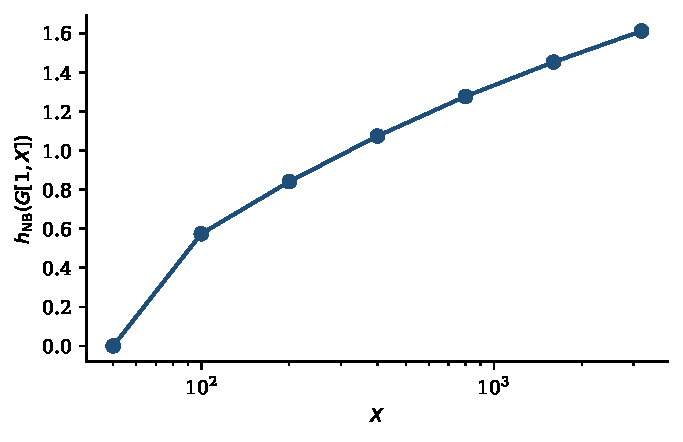
\includegraphics[width=0.6\textwidth]{../figures/fig10_window_entropy.pdf}
\caption{Computed $\hNB(G[1,X])$.}\label{fig:window}
\end{figure}
